\chapter{Introducción}

La \textbf{informática} es un área de la ciencia que abarca distintas disciplinas teóricas (como la creación de algoritmos, teoría de computación, teoría de la información, ...) y disciplinas prácticas (diseño de hardware, implementación de software).

A la hora de crear programas (o \textit{software}), podemos identificarlos de distintos tipos:
\begin{itemize}
    \item \textbf{Software de sistema}: Programas o aplicaciones que pertenecen al sistema y nos ayudan a mejorarlo, administrarlo ... Pueden ser aplicaciones de monitorización, de auditoría de logs, \textit{drivers}, ...

    \item \textbf{Software de desarrollo}: En este caso serán aplicaciones que nos ayudarán a crear otras aplicaciones. Por ejemplo: librerías de funciones, compiladores, \textit{debuggers}, IDEs...

    \item \textbf{Aplicaciones de usuario}: Son aplicaciones que los usuarios finales utilizarán en su día a día. Podríamos diferenciarlas como:
    \begin{itemize}
        \item \textbf{Aplicaciones generalistas}: Son aquellas que cualquier tipo de usuario utilizará en cualquier momento. Son creadas con un propósito específico, pero que no hay que tener grandes conocimientos para usarlas. Por ejemplo: navegadores web, clientes de correo, aplicaciones de ofimática simple, calculadora, calendario, ...

        \item \textbf{Aplicaciones de uso específico}: En este caso son aplicaciones creadas para un usuario específico, con una utilidad muy concreta y que normalmente deben existir conocimientos para utilizarla.

        Pueden ser aplicaciones no muy complejas, pero cuya utilidad, o lo que hagan, tenga importancia y conste de procesos complejos. Por ejemplo: aplicaciones CAD, sistemas de virtualización, aplicaciones científicas (R, JupyterLab), aplicaciones empresariales, ...
    \end{itemize}
\end{itemize}

En esta asignatura veremos distintos tipos de software especializado dentro de la gestión empresarial como son los ERP y los CRM, que podríamos englobar como \textbf{sistemas de información}.

\chapter{Sistemas de información}

Un sistema de información, de manera generalizada, es aquel que ayuda a administrar, recolectar, recuperar, procesar, almacenar y distribuir información relevante para ser usados dentro de los procesos fundamentales de una organización.

Normalmente estos sistemas de información son fáciles de usar, tienen cierto grado de flexibilidad (se pueden adaptar a las empresas), permiten guardar y recuperar información de manera rápida y sencilla.

De esta manera, la información resultante será más valiosa para la propia organización, ya que tendrá una “imagen” más amplia y habiendo podido relacionar más información que de no haber utilizado este tipo de software.

\section{Componentes}
Un sistema de información debe contar con los siguientes componentes básicos, que deben interactuar entre sí de manera adecuada para un buen funcionamiento global:
\begin{itemize}
    \item El \textbf{hardware}, equipo físico utilizado para procesar y almacenar datos.
    \item El \textbf{software} y los procedimientos utilizados para transformar y extraer información.
    \item Los \textbf{datos} que representan las actividades de la empresa.
    \item La \textbf{red} que permite compartir recursos entre computadoras y dispositivos.
    \item Las \textbf{personas} que desarrollan, mantienen y utilizan el sistema.
\end{itemize}

El último punto es muy importante, ya que de nada sirve tener la mejor herramienta, en el mejor hardware, si luego las personas que van a hacer uso de ella no tienen los conocimientos suficientes.

\errorbox{\textbf{Las personas que utilizan los sistemas de información deben tener los conocimientos adecuados para su correcta utilización.}}

Es por eso que las personas que hagan uso del sistema de información deberán ser entrenadas y/o tener manuales para su correcto uso, así como \textbf{también tener en cuenta sus opiniones para mejorar los procesos internos de la empresa}.

\section{Datos vs información}

Los datos reflejan hechos recogidos en la organización y que están todavía sin procesar (reflejan valores o resultados de mediciones). Estos datos serán hechos o cifras sobre algún tema específico concreto, que a simple vista no tienen por qué decir nada.

Por otro lado, la información se obtiene una vez se han procesado, agregado y/o presentado de manera adecuada esos datos para que puedan ser útiles y de esta manera obtener un valor que de otra manera no se podría obtener.

El ejemplo más claro entre datos e información se puede obtener en cualquier \textbf{estudio científico}, en el que a tras la obtención de unos datos, a través del método científico se llega una conclusión y con ello información.

Por ejemplo, mediciones del dióxido de carbono (CO$_{2}$) en la atmósfera, se obtienen  datos y se llega a la siguiente imagen que es la información:

\begin{center}
    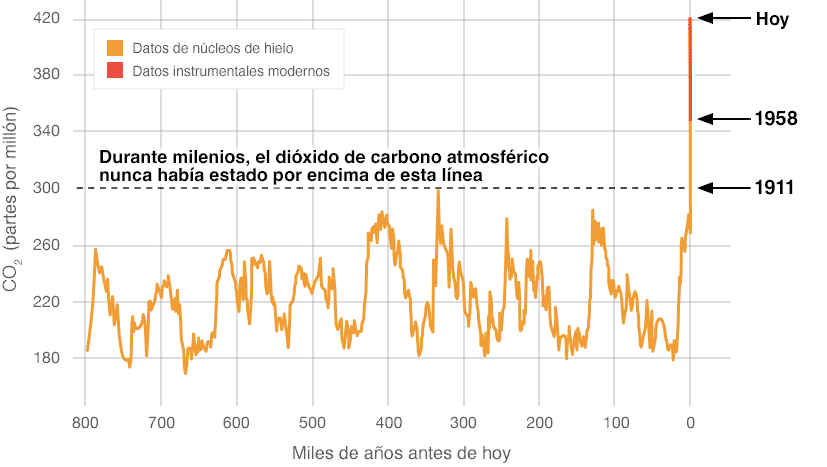
\includegraphics[width=0.7\linewidth]{co2.png}
    \captionof{figure}{Mediciones de CO$_{2}$ en los últimos miles de años. Fuente: \href{https://climate.nasa.gov/en-espanol/signos-vitales/dioxido-de-carbono/}{NASA}.}
\end{center}



\section{Objetivo}

El objetivo de los sistemas de información, y en este caso, los utilizados para la gestión empresarial, es el de realizar acciones de manera más rápida y eficiente, por lo que también debería ser más económico para la empresa.

El uso de las tecnologías de la información y la comunicación en las empresas se ha convertido en un \textbf{elemento esencial como motor vertebrador y fuente de ventajas competitivas}.

Hoy en día una empresa que no haga uso de la informática está condicionando su estrategia empresarial, y es bastante probable que esté perdiendo oportunidades de negocio, así como la posibilidad de desarrollar sus productos y servicios.

Es por eso que el uso de la informática y de \textit{software} especializado de gestión empresarial puede ayudar a las empresas en:

\begin{itemize}
    \item Obtener ventajas competitivas.
    \item Mejorar la eficiencia interna de la empresa: reducir costes, mejorar la productividad, mejorar la organización de la información, ...
    \item Mejorar y facilitar la toma de decisiones a través de la recopilación de la información.
    \item Para desarrollar nuevas estrategias de negocios.
\end{itemize}

\section{Requisitos}

Para que la información sea útil en la toma de decisiones dentro de una organización, debe cumplir una serie de requisitos:

\begin{itemize}
    \item \textbf{Exactitud}: debe ser precisa y libre de errores.
    \item \textbf{Comprensión}: inteligible por el usuario.
    \item \textbf{Completitud}: debe contener todos aquellos hechos que pudieran ser importantes.
    \item \textbf{Economicidad}: el coste para obtener la información debe ser menor que el beneficio.
    \item \textbf{Confianza}: garantizar tanto la calidad de los datos utilizados, como la de las fuentes de información.
    \item \textbf{Relevancia}: ha de ser útil para la toma de decisiones.
    \item \textbf{Nivel de detalle}: se debe proporcionar con la presentación y el formato adecuados, para que resulte sencilla y fácil de manejar.
    \item \textbf{Oportunidad}: se debe entregar la información a la persona que corresponde y en el momento adecuado.
    \item \textbf{Verificabilidad}: la información ha de poder ser contrastada y comprobada en todo momento.
\end{itemize}

\warnbox{A tener en cuenta: \textbf{el exceso de información también puede ser contraproducente}.}


\chapter{ERP}
Los sistemas de planificación de recursos empresariales (\textbf{ERP}, por sus siglas en inglés, \textit{enterprise resource planning}) son los sistemas de información gerenciales que integran y manejan muchos de los negocios asociados con las operaciones de producción y de los aspectos de distribución de una compañía en la producción de bienes o servicios.




\chapter{CRM}


\chapter{Arquitectura de servicios}

todo en un servidor, por capas...